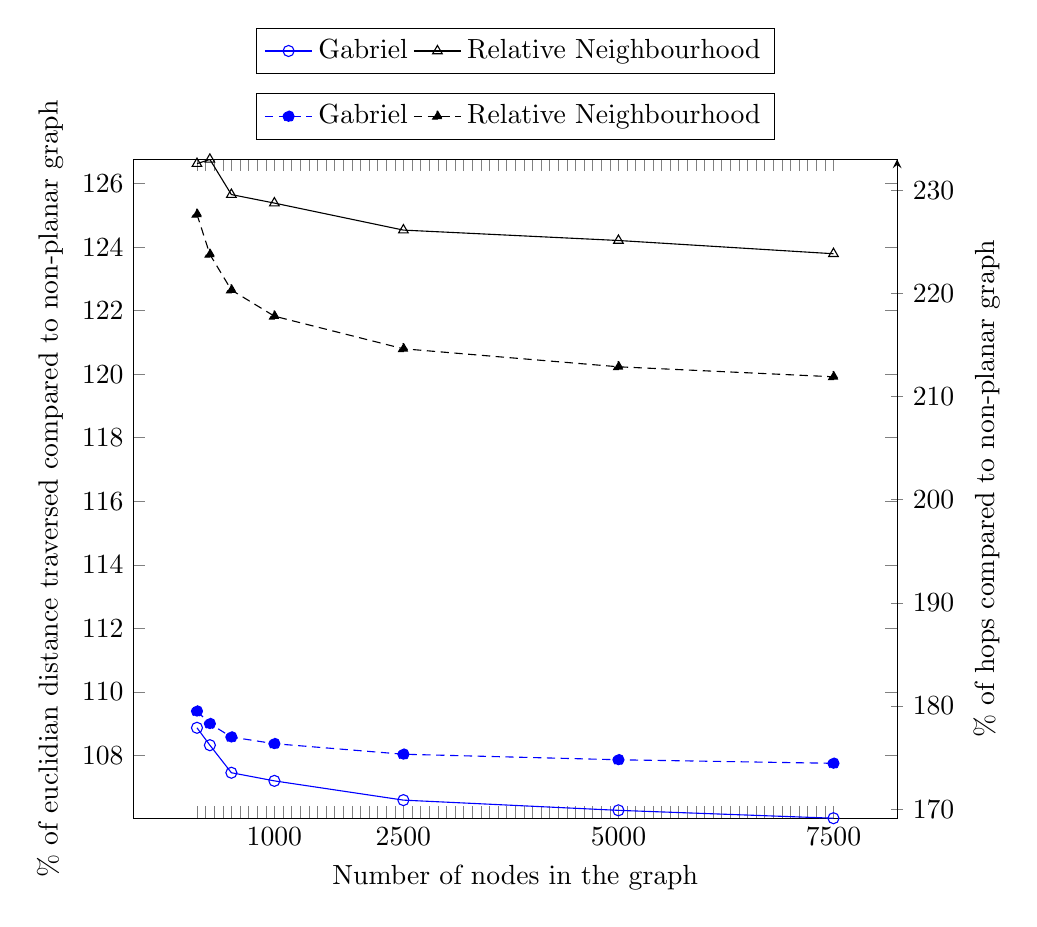
\begin{tikzpicture}
\pgfplotsset{every axis legend/.append style={at={(0.5,1.03)},anchor=south}, }
\begin{axis}[scale only axis, xtick={100, 200, 300, 400, 500, 600, 700, 800, 900, 1000, 1100, 1200, 1300, 1400, 1500, 1600, 1700, 1800, 1900, 2000, 2100, 2200, 2300, 2400, 2500, 2600, 2700, 2800, 2900, 3000, 3100, 3200, 3300, 3400, 3500, 3600, 3700, 3800, 3900, 4000, 4100, 4200, 4300, 4400, 4500, 4600, 4700, 4800, 4900, 5000, 5100, 5200, 5300, 5400, 5500, 5600, 5700, 5800, 5900, 6000, 6100, 6200, 6300, 6400, 6500, 6600, 6700, 6800, 6900, 7000, 7100, 7200, 7300, 7400, 7500}, xticklabels={, , , , , , , , , $1000$, , , , , , , , , , , , , , , $2500$, , , , , , , , , , , , , , , , , , , , , , , , , $5000$, , , , , , , , , , , , , , , , , , , , , , , , , $7500$}, legend columns=4,width=0.8\linewidth, xlabel=Number of nodes in the graph, ylabel=\% of euclidian distance traversed compared to non-planar graph]
\addplot[color=blue, mark=*, densely dashed] coordinates{
(100, 109.394763995)
(250, 109.000974877)
(500, 108.579684211)
(1000, 108.370662895)
(2500, 108.038634263)
(5000, 107.864608408)
(7500, 107.75284513)
};
\addplot[color=black, mark=triangle*, densely dashed] coordinates{
(100, 125.032037309)
(250, 123.77048413)
(500, 122.649392264)
(1000, 121.825884888)
(2500, 120.800217485)
(5000, 120.233295306)
(7500, 119.918682611)
};
\legend{Gabriel, Relative Neighbourhood}
\end{axis}

\pgfplotsset{every axis legend/.append style={at={(0.5,1.20)},anchor=north}}
\begin{axis}[scale only axis, width=0.8\linewidth, legend columns=4, axis y line=right, axis x line=none, ylabel=\% of hops compared to non-planar graph]
\addplot[color=blue, mark=o] coordinates{                
(100, 177.883127848)
(250, 176.196812205)
(500, 173.526897693)
(1000, 172.737217416)
(2500, 170.871355665)
(5000, 169.88022916)
(7500, 169.116950299)
};
\addplot[color=black, mark=triangle] coordinates{                
(100, 232.574847787)
(250, 232.985044361)
(500, 229.577034364)
(1000, 228.751954654)
(2500, 226.133052768)
(5000, 225.125269594)
(7500, 223.840863379)
};
\legend{Gabriel, Relative Neighbourhood}
\end{axis}
\end{tikzpicture}
